
\section{Examples}

\lstset{ %
frame=single,                   % adds a frame around the code
tabsize=2,                      % sets default tabsize to 2 spaces
captionpos=b,                   % sets the caption-position to bottom
breaklines=true,                % sets automatic line breaking
}

\subsection{Example 1: hello world}

This example program is a simple "hello world" program, as this was practically
the only program that was able to pass through the entire pipeline. Following
is the "hello world" program written in Haskell:

\begin{footnotesize}
\lstinputlisting[language=Haskell]{"../interpreter/tests/helloworld.hs"}
\end{footnotesize}

\subsubsection{Converted to Core}

After the program has passed through GHC and the external-core file
has been generated, the program looks like this:

\begin{footnotesize}
\lstinputlisting{"../interpreter/tests/helloworld.hcr"}
\end{footnotesize}

... TODO: Explain this representation in more detail.

\subsubsection{Converted to JSCore}

In the next step it is parsed and dumped to JSCore:

\begin{footnotesize}
\lstinputlisting{"../interpreter/tests/helloworld.hcj"}
\end{footnotesize}

\subsubsection{JSCore graph}

Using the parsing libraries of PyPy we can generate a nice graph from the result,
directly corresponding to the resulting datastructure. 
See figure \ref{fig:helloworldgraph}.
By simply traversing this datastructure we can generate the AST for the Core 
interpreter (Haskell-Python).

\begin{sidewaysfigure}
\begin{figure}[H]
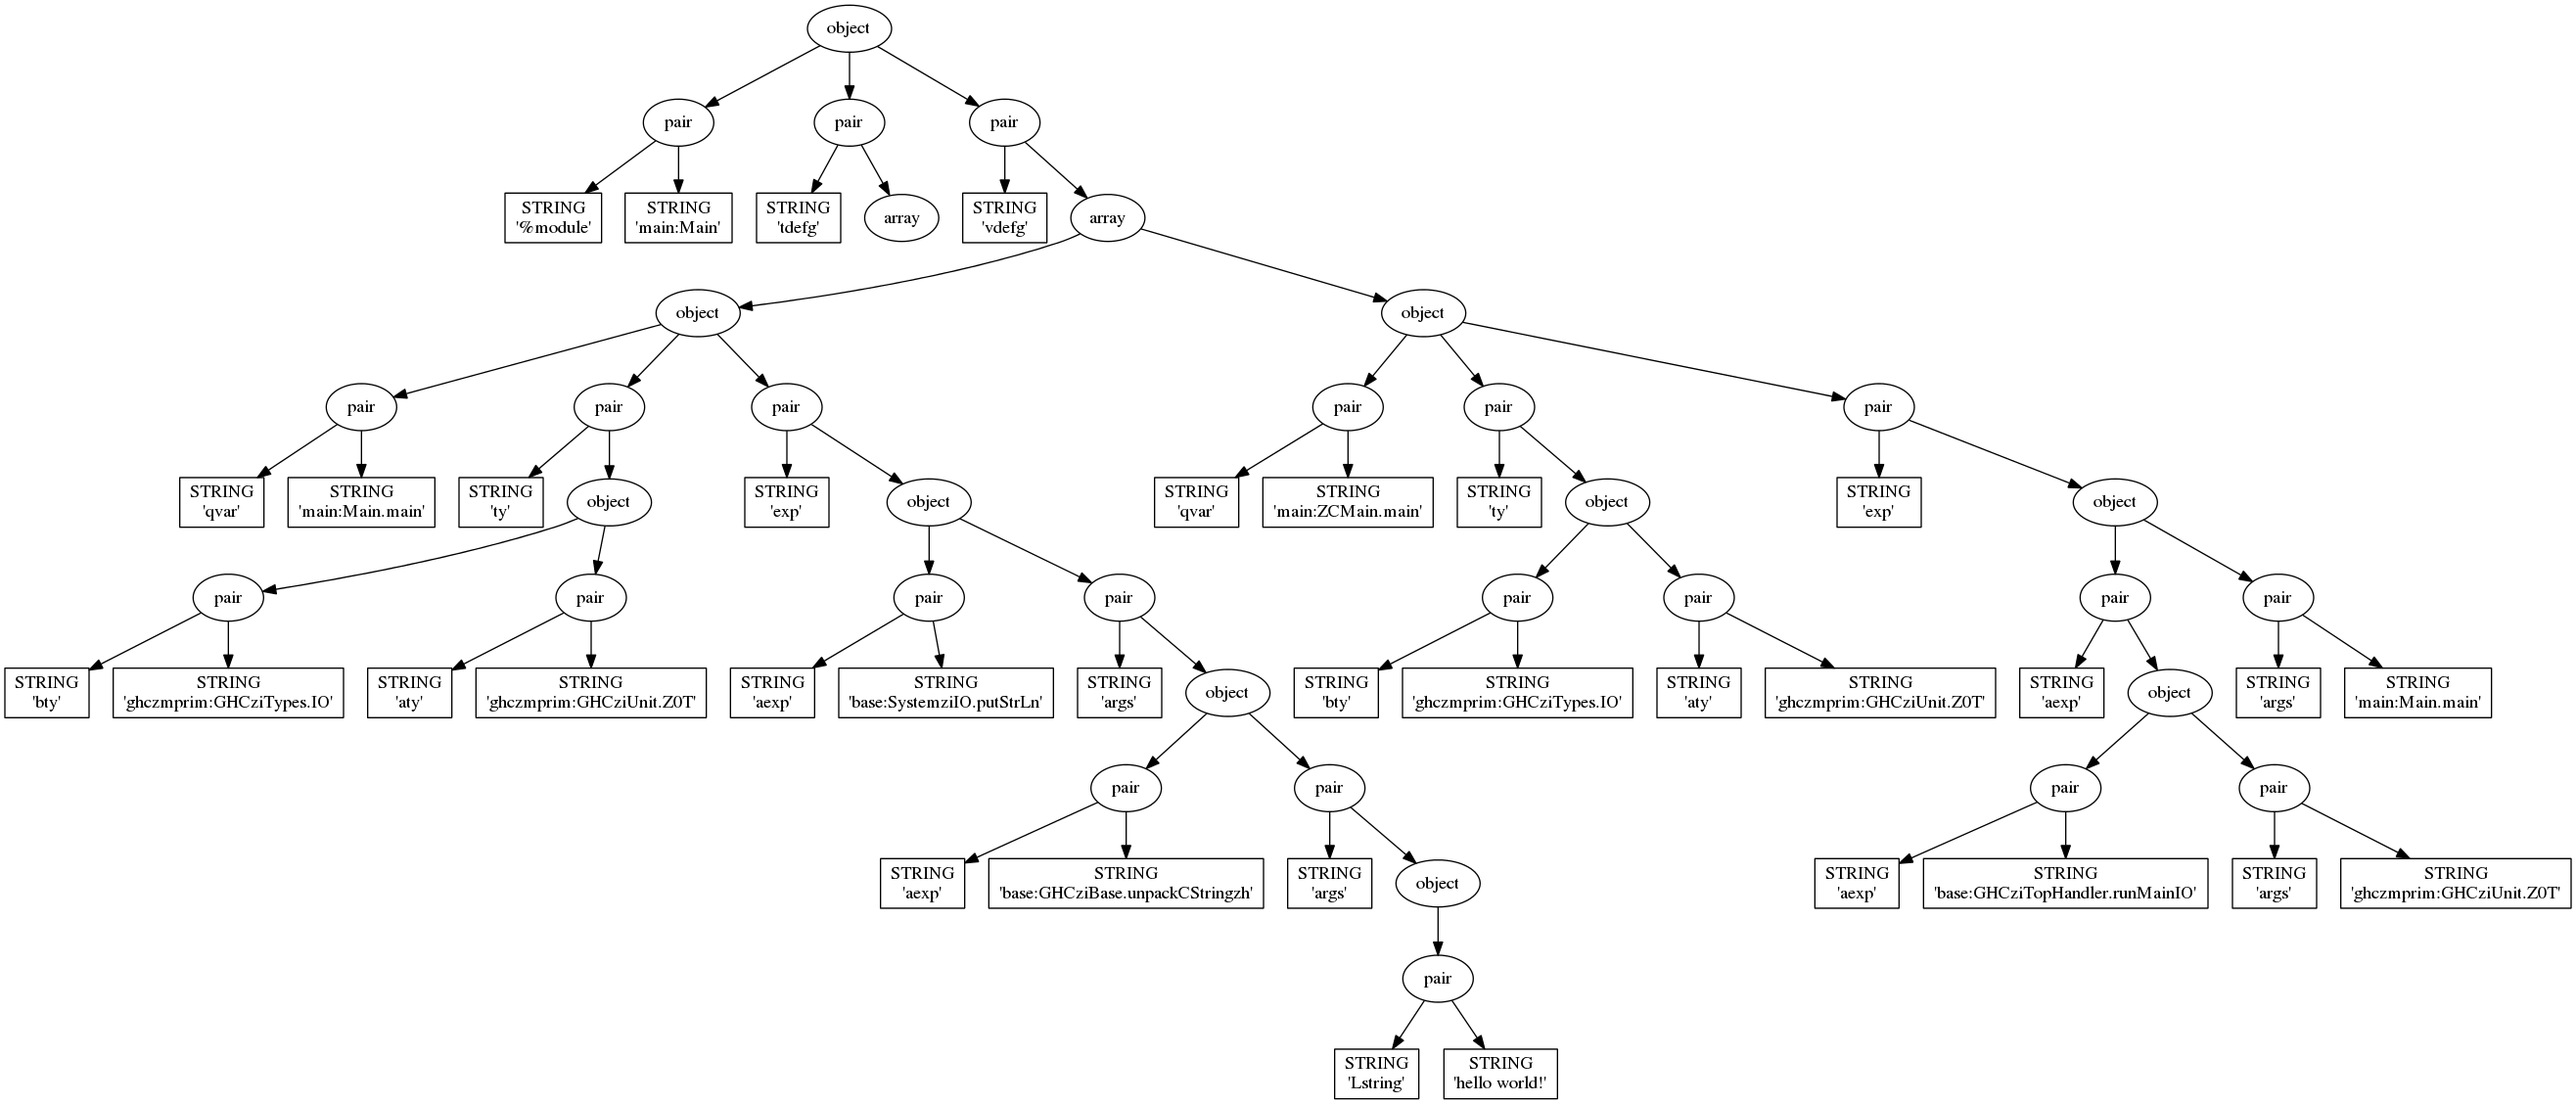
\includegraphics[width=\textwidth]{../interpreter/tests/helloworld.png}
\caption{Example program translated to JSON}
\label{fig:helloworldgraph}
\end{figure}
\end{sidewaysfigure}

\subsubsection{Result}

The program results as expected, outputting the string "Hello, world!".

\begin{comment}

\subsection{Example 2: naive fibonacci}

The following program is a simple fibonacci program.

\begin{footnotesize}
\lstinputlisting[language=Haskell]{"../interpreter/tests/fib.hs"}
\end{footnotesize}

\subsubsection{Converted to Core}

As we can see, the simple hello world program becomes more complex when translated
to Core by GHC.

\begin{footnotesize}
\lstinputlisting{"../interpreter/tests/fib.hcr"}
\end{footnotesize}

%TODO: Explain this representation in more detail.

\subsubsection{Converted to JSCore}

And translated to JSCore by our serializer:

\begin{footnotesize}
\lstinputlisting{"../interpreter/tests/fib.hcj"}
\end{footnotesize}

\subsubsection{JSCore graph}

Using the parsing libraries of PyPy we can generate a nice graph from the result, 
see figure \ref{fig:fibgraph}

By simply traversing this datastructure we can generate the AST for the Core interpreter.

\begin{sidewaysfigure}
\begin{figure}[H]
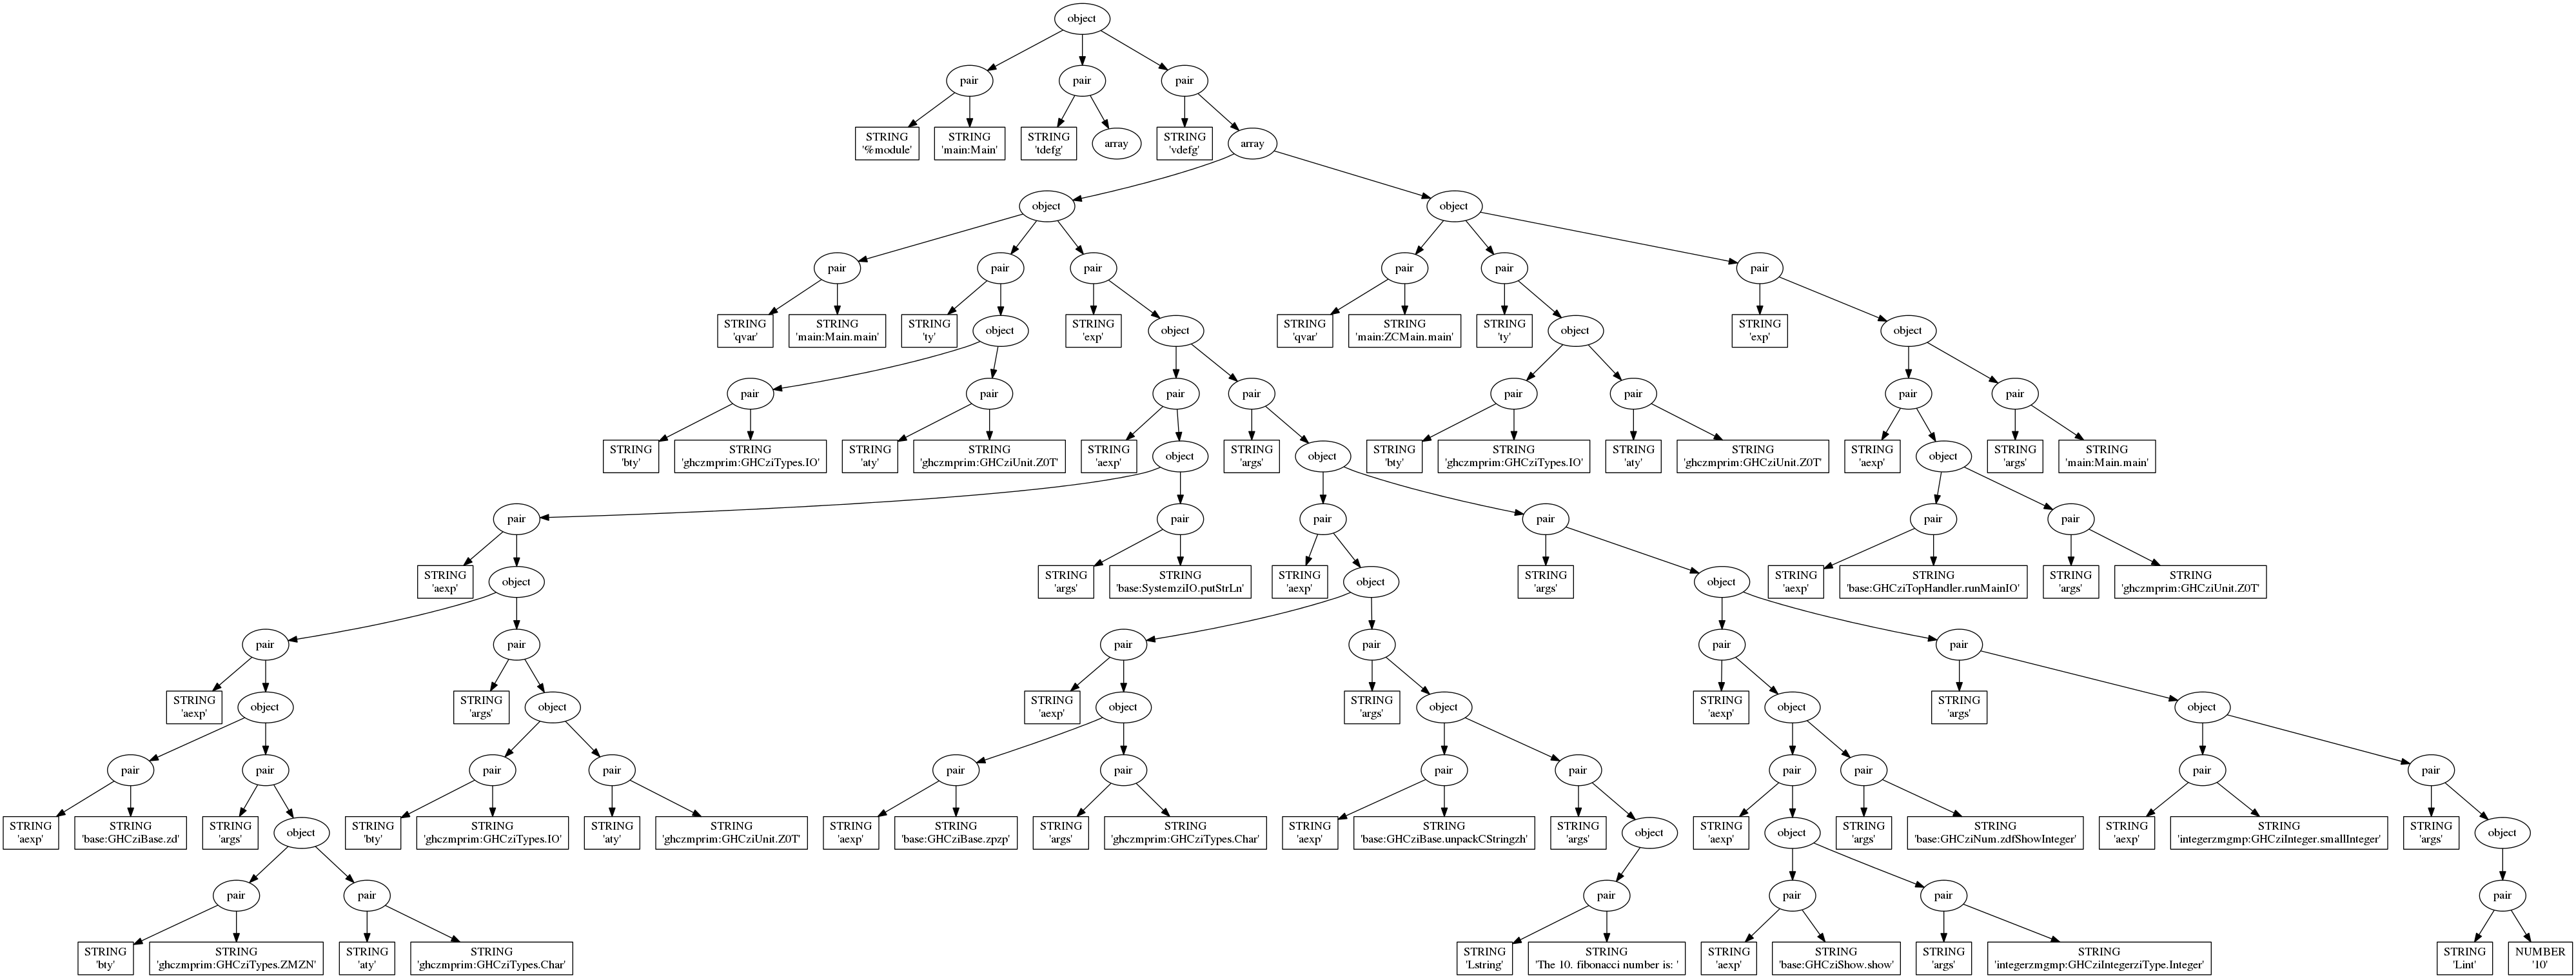
\includegraphics[width=\textwidth]{../interpreter/tests/fib.png}
\caption{Example program 2 translated to JSON}
\label{fig:fibgraph}
\end{figure}
\end{sidewaysfigure}

\subsubsection{Result}

\end{comment}
